\documentclass{article}
\usepackage[dblblindworkshop]{neurips_2026}
\usepackage{amsmath,booktabs,graphicx,microtype}
\title{When Evaluation Cues Become the Evaluation: Supplementary Material}
\author{Anonymous Workshop Submission}
\workshoptitle{TAE (Trust-AI-Eval): Can We Trust AI Evaluation?}
\begin{document}
\maketitle

\section{Evidence and provenance}
The primary freeze is the full320-v3 dataset at the pinned revision recorded in \texttt{provenance/full320-v3/hf\_snapshot.json}. It contains 11,520 rendered rows from 320 payload blocks. Every activation result used for the main figures is copied into \texttt{artifacts/pinned\_full320/}; the submission figure hashes and claim restrictions are recorded in \texttt{artifacts/submission\_figure\_manifest.json}. The equal-training-size development control is \texttt{artifacts/full320\_equal\_n\_llama31\_8b\_l12.json}.

\section{Complete observational figure set}
\begin{figure}[h]
\centering
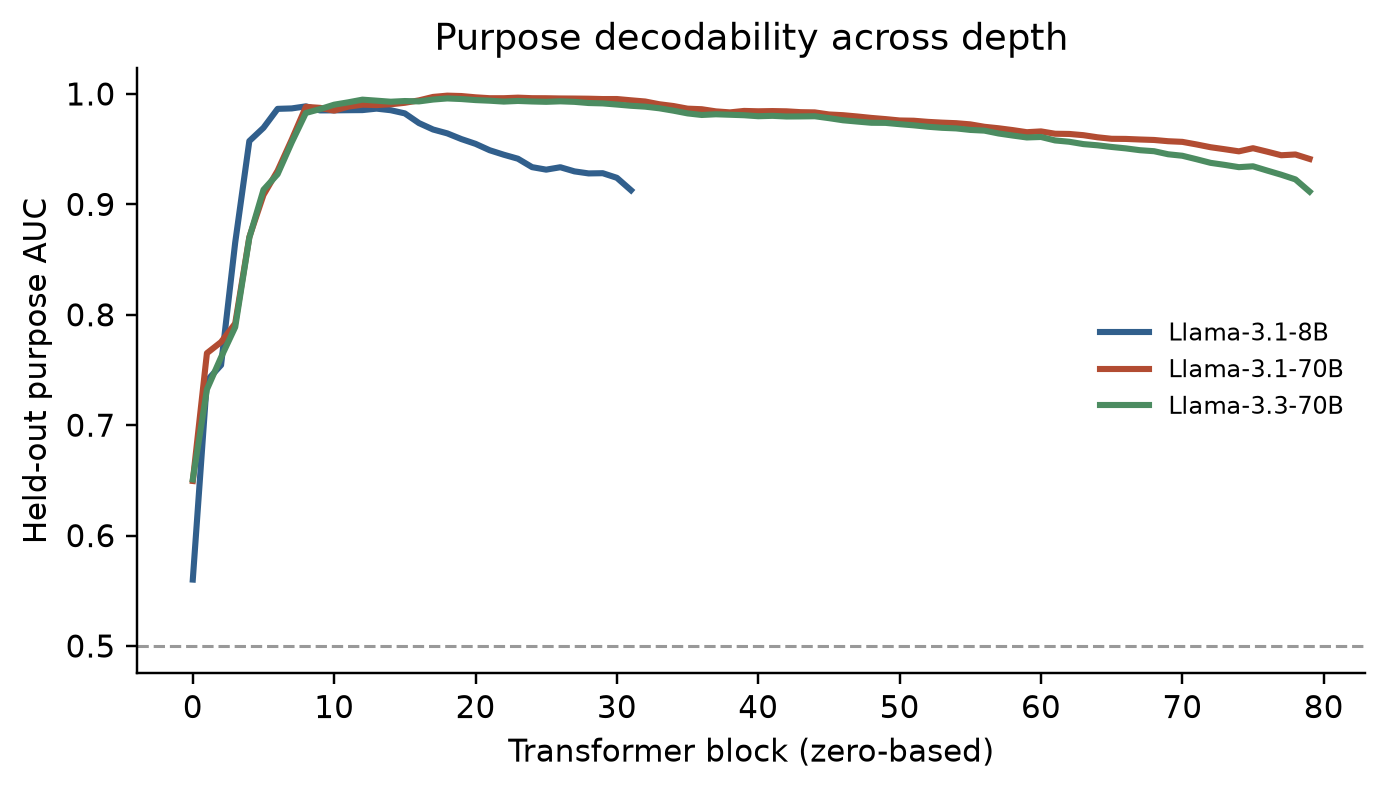
\includegraphics[width=.95\linewidth]{figures/main_purpose_by_depth.png}
\caption{Held-out purpose AUC across depth for the three pinned model result files.}
\end{figure}
\begin{figure}[h]
\centering
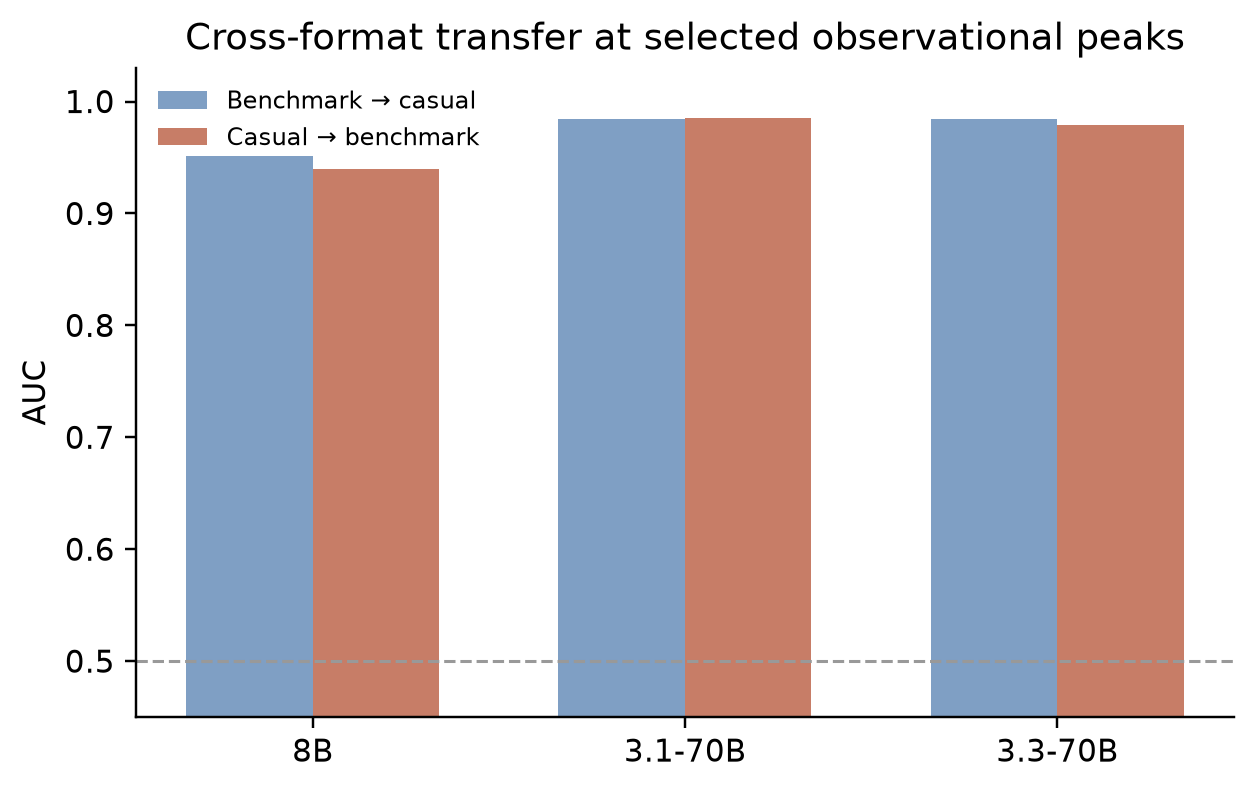
\includegraphics[width=.95\linewidth]{figures/main_cross_format_transfer.png}
\caption{Cross-format transfer at descriptive observational peaks.}
\end{figure}
\begin{figure}[h]
\centering
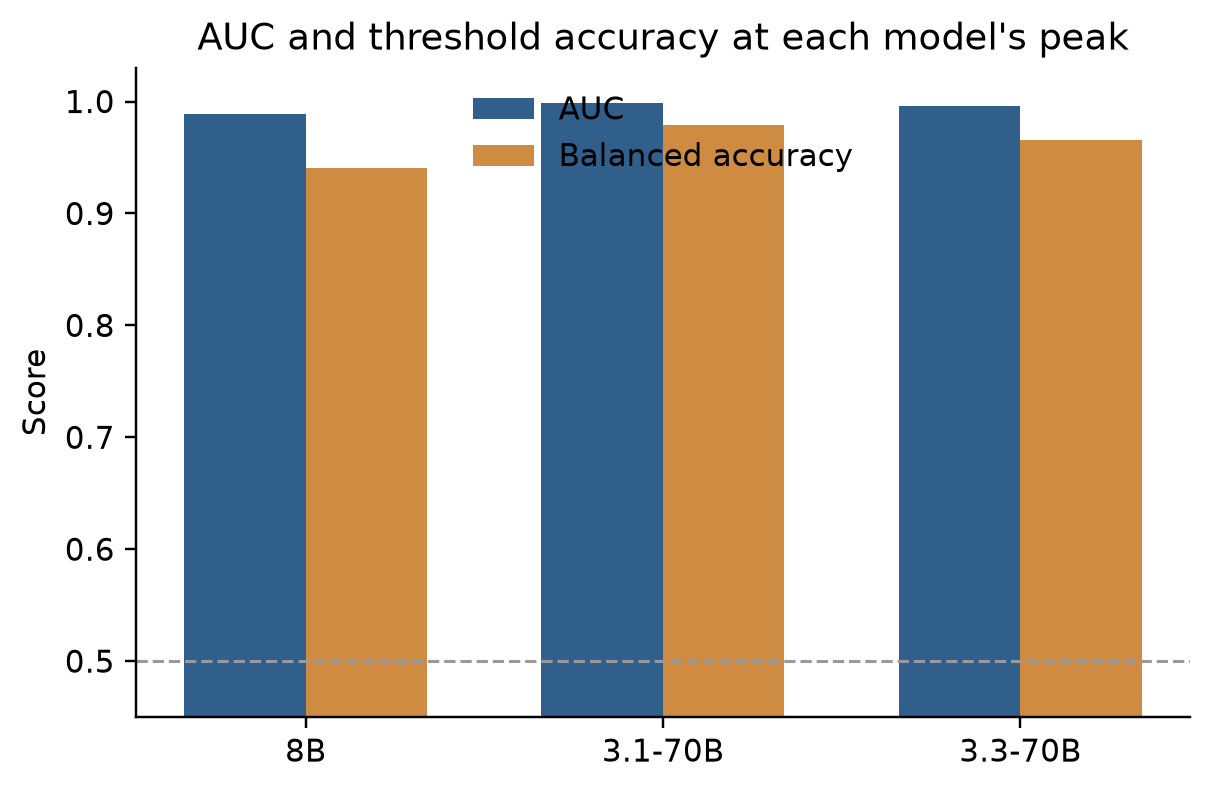
\includegraphics[width=.95\linewidth]{figures/main_auc_balanced_accuracy.png}
\caption{AUC and balanced accuracy at descriptive peaks.}
\end{figure}

\section{Equal-N and direct diagnostic controls}
\begin{figure}[h]
\centering
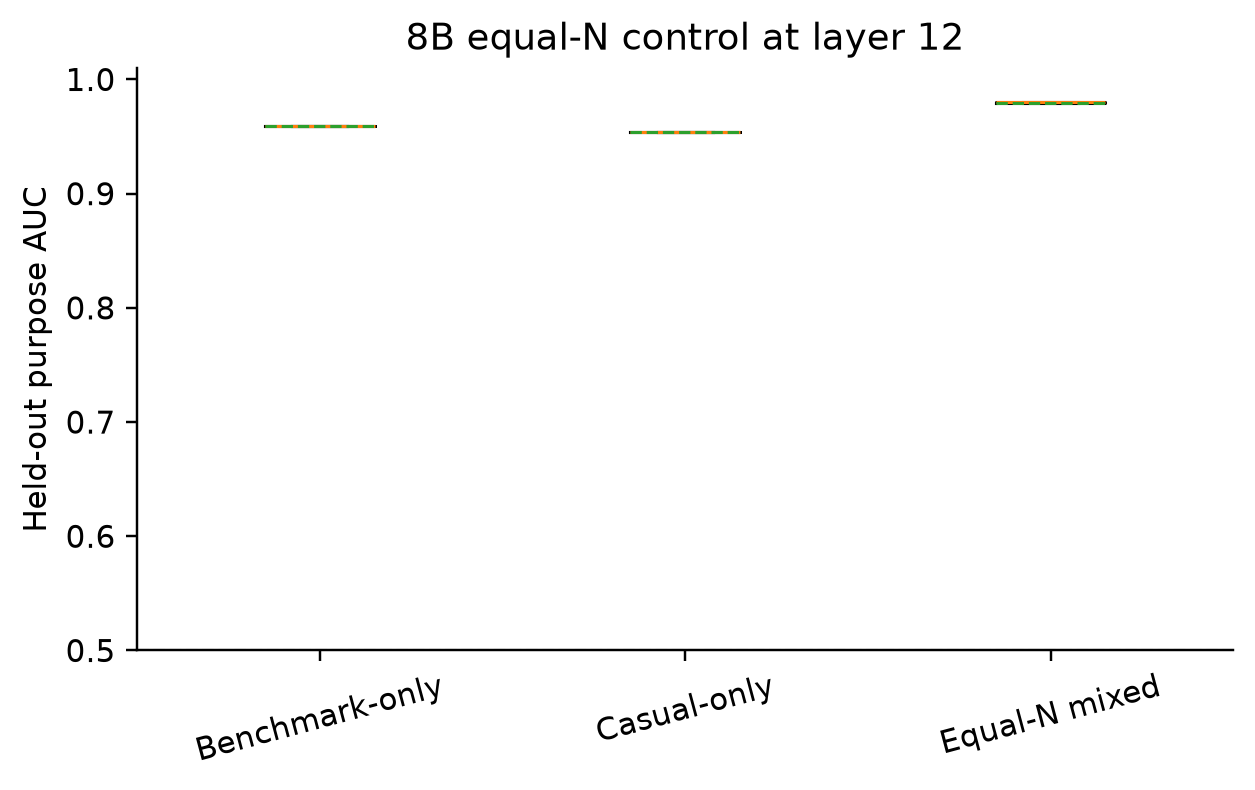
\includegraphics[width=.95\linewidth]{figures/main_equal_n_8b.png}
\caption{Four-seed 8B equal-training-size control at layer 12. This is not an all-model replication.}
\end{figure}
\begin{figure}[h]
\centering
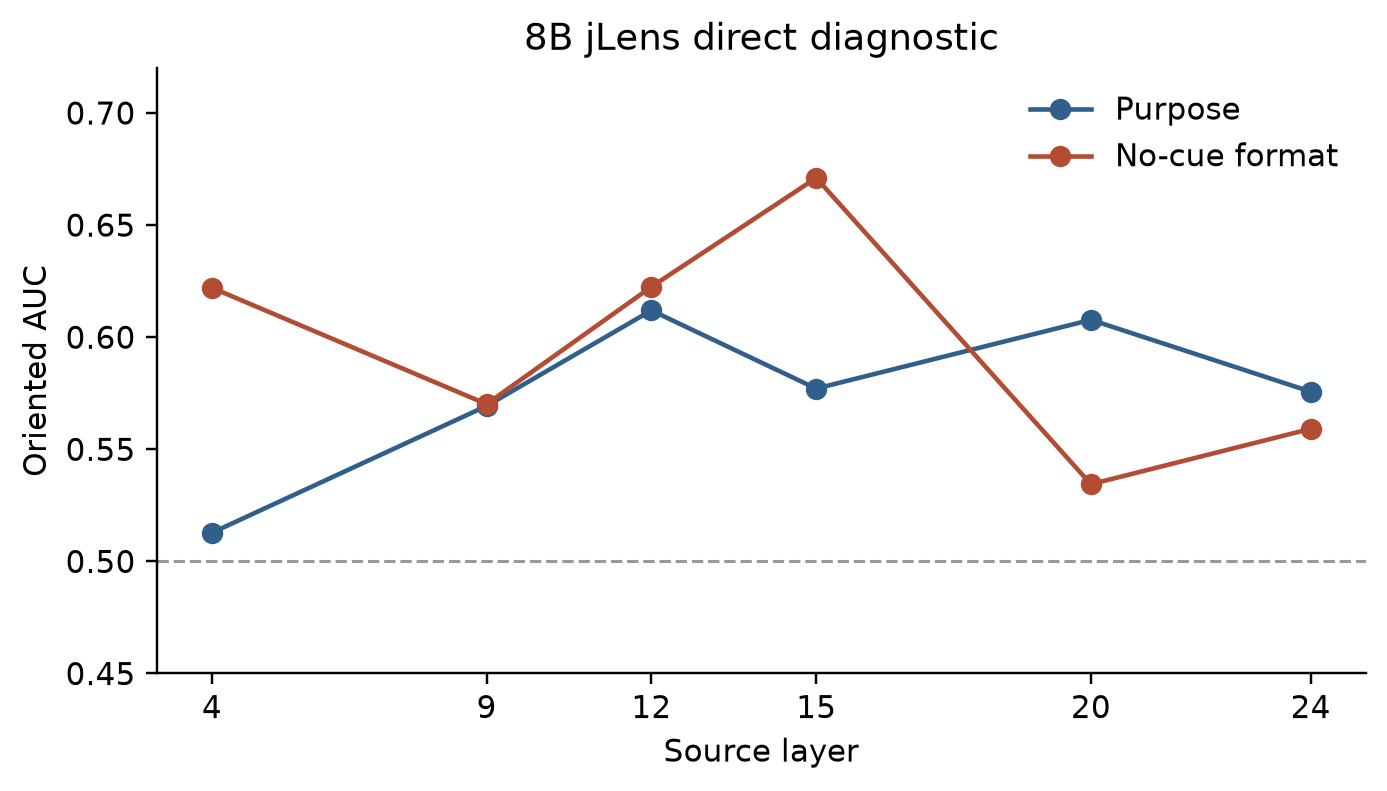
\includegraphics[width=.95\linewidth]{figures/appendix_jlens_direct_diagnostic.png}
\caption{Development-only 8B Jacobian-lens direct diagnostic.}
\end{figure}

\section{Claim restrictions}
These artifacts support observational stated-purpose decodability and protocol auditing. They do not establish evaluation awareness, behavioral steering, causal intervention, confirmation, or a scale effect. The pilot80-v2 and devbunova datasets are separate freezes and are not pooled with full320-v3. The equal-N control and direct lens are currently 8B-only.

\end{document}
